\subsubsection*{Methodology of the DET subproject}

\paragraph{Construction and commissioning of P0 and P4:}

\begin{figure}[!htb]
	\centering
	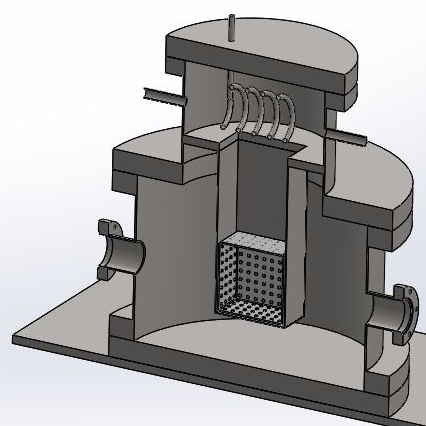
\includegraphics[scale=0.4]{img/P0.png}
	\caption{\label{fig.P0} Conceptual sketch of P0.  }
\end{figure}

\begin{figure}[!htb]
	\centering
	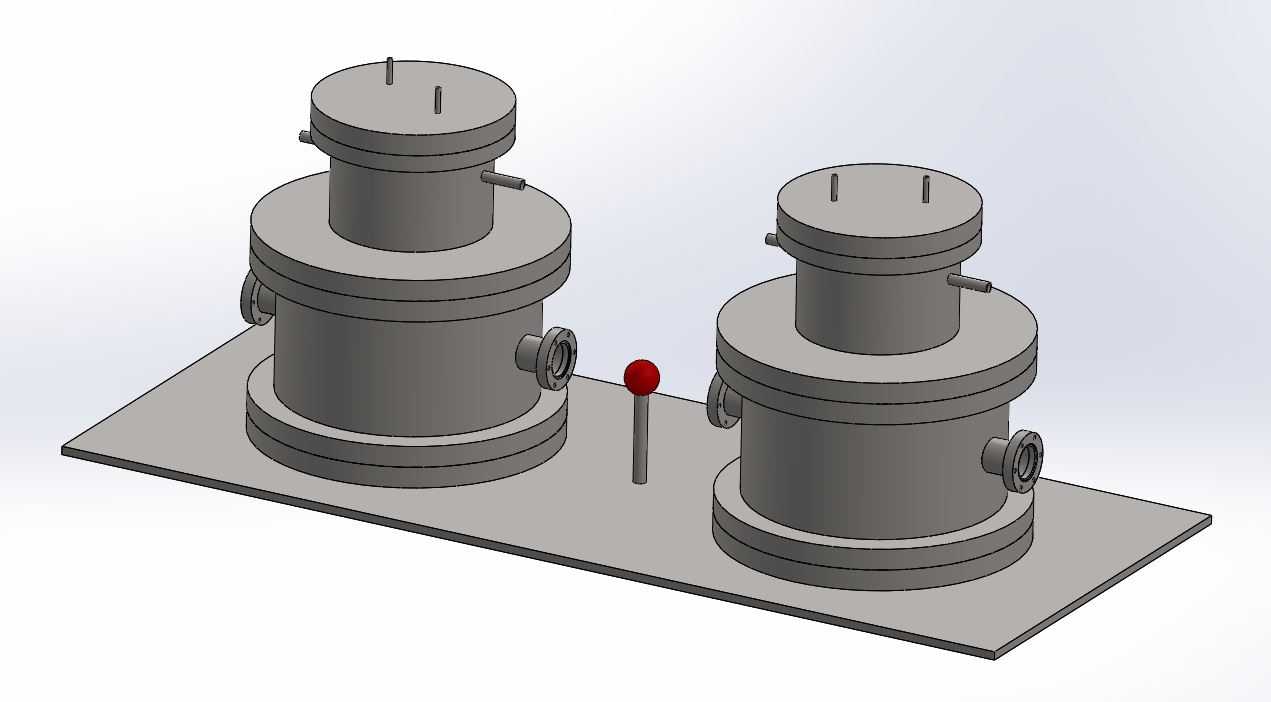
\includegraphics[scale=0.4]{img/P2.JPG}
	\caption{\label{fig.P2} Conceptual sketch of P4. The red sphere in the middle represents the phantom used for imaging reconstruction.}
\end{figure}

PETALO-0 (P0) will be a demonstrator used to study the intrinsic performance of the LXSC. Figure \ref{fig.P0} shows a conceptual sketch. A fully instrumented LXSC6, immersed in its own cryostat will be studied with a radioactiva source emitting 511 keV photons, such as Na-22 (eventually other sources will be used to study the linearity of the system). The redundancy of LXSC6 will allow to measure the energy and spatial resolution from the data themselves. In addition, P0 will be used to understand the energy and time triggers of the device. 

PETALO-4 is a demonstrator of the PETALO concept using 4 LXSC arranged in groups of two facing each other. The system can be designed with two independent cryostats (each cryostats holds two cells), as shown in Figure \ref{fig.P2} to permit maximum flexibility in the placement and arrangement of the device. P4 will be used to reconstruct images from phantoms and eventually small animals, in order to demonstrate the imaging reconstruction capabilities of PETALO as well as its potential as TOF device. 

%\begin{figure}[!htb]
%	\centering
%	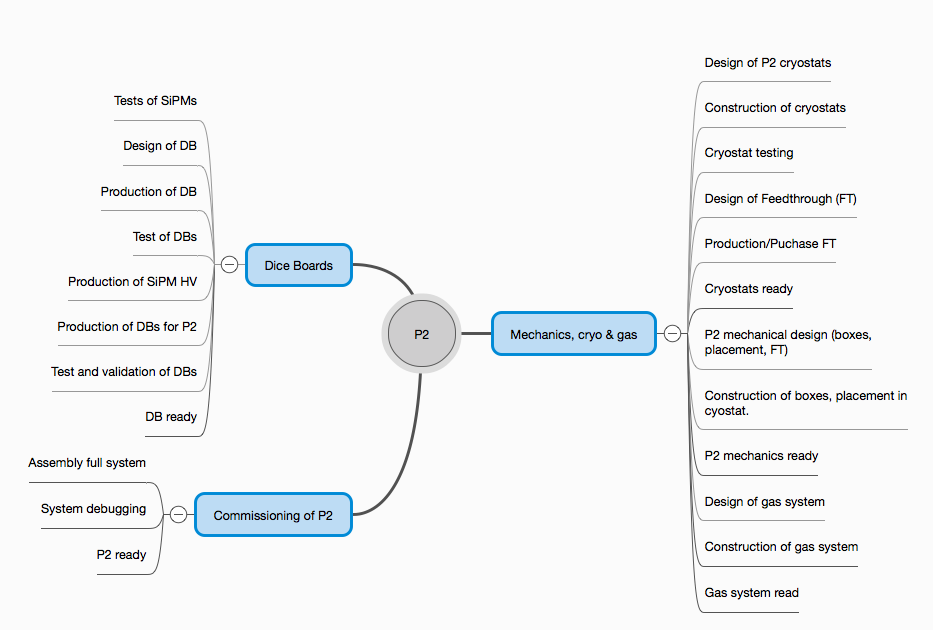
\includegraphics[scale=0.5]{img/P2MIND.png}
%	\caption{\label{fig.P2MIND} Conceptual breakdown of activities for the construction of P0 and P4.  }
%\end{figure}

\begin{figure}[!htb]
	\centering
	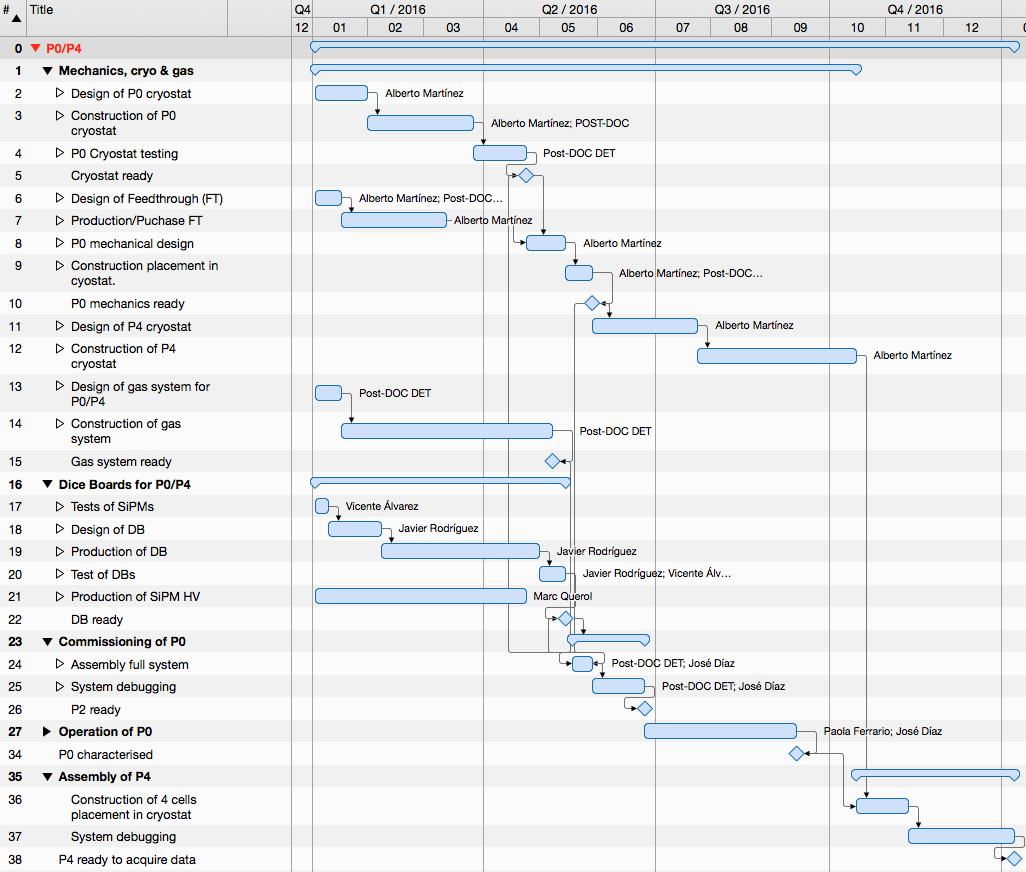
\includegraphics[scale=0.5]{img/P4WF.png}
	\caption{\label{fig.P2WF} Work flow of activities for P2/P4.  }
\end{figure}

The construction of P0 and P4 involve a number of activities  organised in three groups: (i) Mechanics, cryogenics and gas system (MCG);  (ii) Dice Boards for P0 and P4 (DB);  and assembly, commissioning and operation (ACP) for P0 and P4. 

The MCG group includes the design, construction and tests of the cryostats; the design and construction of the feedthroughs (FT) needed to extract the signals from the DB to the digitising electronics located outside the cryostats (the FT will be of the same time used for the NEXT tracking plane and manufactured by the same company that was employed by NEXT);  and the design and construction of ancillary mechanics. The DB group includes the design, production and test of the DB (which will be straight-forward modifications of the DB used in the NEXT tracking plane, and manufactured by the same company employed by NEXT), the production of the SiPM high-voltage modules (these have been developed by NEXT and PETALO will only need to pay for an extra production of modules), and the testing and assembly of the full system. The ACP group includes the activities related with the commissioning and operation of the deviaces. A detailed work flow (WF) is shown in Figure \ref{fig.P2WF}. The WF, including dependencies of tasks yields a schedule for the construction of P2 that encompassed the first two quarters of 2016 (we denote this as Q1/Q2-16). 

\paragraph{Operation of P0:}

%\begin{figure}[!htb]
%	\centering
%	\includegraphics[scale=0.5]{img/EnergyCor2P2.png}
%	\caption{\label{fig.ECP2} Dependence of the energy measured in P2 wit the transverse (x) and longitudinal (z) coordinate. A small position dependence is observed.   }
%\end{figure}

P0 will demonstrate the excellent resolution of the system in energy, position and time. A \NA\ source, located between the two modules will emit back-to-back gammas, which will be the primary calibration source of the detector. 

The plan of measurements include:
\begin{enumerate}
\item {\bf Study of the energy resolution using photoelectric events.} Photoelectric events are easily characterised in the LXSC, as single-site deposition events (unless conventional SSDs, the LXSC can separate multiple-site events to an expected resolution of a few mm). Then, the energy in the LXSC is measured by adding the signal of all the SiPMs. The energy resolution is obtained by fitting the photoelectric peak. The energy resolution of the LXSC6 will be measured as reference (an energy resolution of better than 3\% FWHM is expected). Then, the energy resolution of the LXSC2 will be measured. A resolution better than 5\% FWHM is expected.
\item {\bf Study of the position resolution using photoelectric events.} To estimate the position resolution from data, we will use the LXSC6 which provides 2 redundant measurements of each coordinate. Then, if $\chi_1,\chi_2$~are redundant measurements of a given coordinate, and $\Delta \chi = \chi_2 - \chi_1$~is the difference between them, the $\Delta \chi$ distribution should have mean zero and standard deviation  
$\delta \Delta \chi \sim \sqrt{2} \delta \chi$. To estimate the position resolution of LXSC2, one starts by validating the Monte Carlo simulation of the LXSC, by comparing data and Monte Carlo results for the LXSC6. After demonstrating that the Monte Carlo reproduces correctly the simulation measured with data for the LXSC6, one can use the Monte Carlo to estimate the position resolution of LXSC2. Position resolution in the range of 1-2 mm are expected. 
%\item {\bf Study of the time resolution using photoelectric events.} Coincidence Resolution Time (CRT) will be measured by comparing the time stamp provided by the two opposite LXSC cells. A CRT in the range of 200 ps is expected.
\end{enumerate}

In addition, a program of studies for Compton interactions (starting with Compton events that deposit their full energy in the cell and show a double-site deposition, will be carried out. The program will include the study of the energy, position and time resolution for double-site Compton events, the study of the resolution to separate double-site events, and the feasibility of using Compton kinematics to improve the resolution of the back projected tracks. 

All the above studies will be lead by Dr. Paola Ferrario, with the help of Post-doc DET and the supervision of the PI. 

\paragraph{Construction and commissioning of P4:}
%
%\begin{figure}[!htb]
%	\centering
%	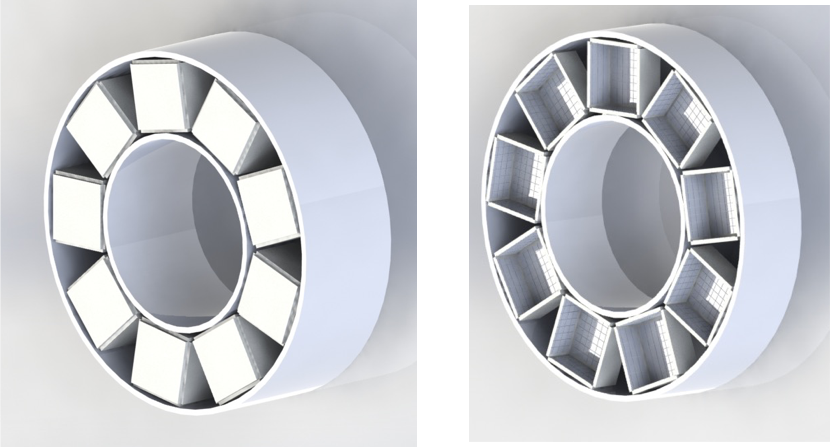
\includegraphics[scale=0.5]{img/SAP.png}
%	\caption{\label{fig.P10} Conceptual sketch of P10.  }
%\end{figure}

PETALO-4 (P4) is a proof-of-concept PET based in 4 independent LXSC2. It will allow the reconstruction of images both from phantoms and from small animals. It will be certified for its use in a hospital (La Fe, Valencia), and will be tested inside the intense magnetic field produced by the NMR research apparatus available at La Fe, to validate the potential operation of PETALO in conjunction with nuclear magnetic resonance.  

%\begin{figure}[!htb]
%	\centering
%	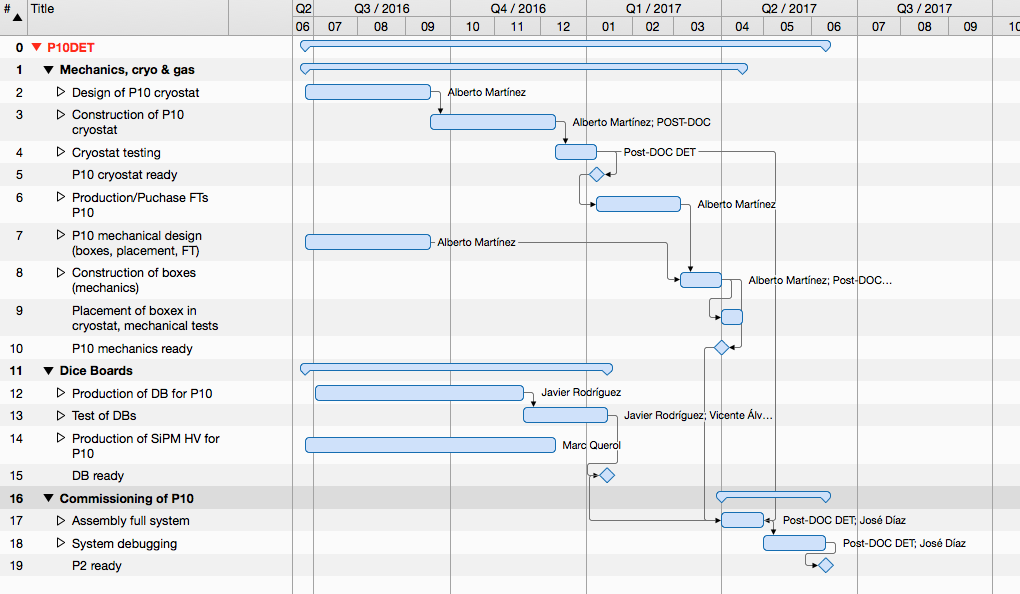
\includegraphics[scale=0.5]{img/P10WF.png}
%	\caption{\label{fig.P10WF} Work flow of activities for the construction of P10.  }
%\end{figure}

P4 will be built reusing 4 of the 6 DB of P0, and therefore only 2 additional DB (and their corresponding electronics) will be needed in addition to those deployed by P0. The construction of the device requires a second (small cryostat), and will use the same gas system than P0 and identical electronics. This permits a very fast time schedule. P0 will be built, commissioned and studied during Q1/Q3-16 and P4 will be ready in Q4-2016. 

%The cells of PETALO will be LXSC2. Production will start after the validation of the LXSC2 design with P2. The PETALO system is scalable, since all the components (DBs, electronic modules) are identical. The gas system is common with P2. The main challenge of P10 is the cryostat. The design of the cryostat will start already in 2016, and will built on the experience of the P2 cryostats. A period of six months is foreseen for the design, followed by six more months for construction. Figure \ref{fig.P10WF} shows the work flow of activities for the construction of P10, which extends from Q2-16 to Q2-17. The activities are similar to those of P2, although the development time has been adjusted to take into account the larger number of cells (DBs) and the complexity of the cryostat design/construction/commissioning. 
% 

\paragraph{SIMPLE and RAP:}
The PETALO simulation (SIMPLE) and software framework analysis (RAP) will be based in existing software developed by the NEXT collaboration. Dr. Ferrario, who has been one of the leading software and analysis developers for NEXT will be fully dedicated to PETALO starting in 2016 and will use her extensive experience to produce working versions of both SIMPLE and RAP by Q2-16. Further development will occur in parallel with the analysis of P4 data, during Q3/Q4-16. This project proposes a FPI student, who will contribute to the software and analysis development (as well as to the operation of P4) working closely with Dr. Ferrario and Prof. J. Díaz.

\paragraph{PETALO as TOF device:}
P4 will allow the measurement of the Coincidence Resolution Time (CRT) by comparing the time stamp provided by the opposite LXSC cells. A CRT in the range of 200-250 ps is expected.The IFIC group will lead the studies related with CRT determination and will participate in the studies of imaging reconstruction using TOF techniques. 

%\paragraph{DET: Summary}
%The DET subproject is in charge of the construction of the P2 and P10 apparatus, as well as of the development of some essential software tools. The construction of P2 will occur during Q1/Q2-16, while the construction of P10 will extend from Q2-16 to Q2-17. Furthermore, during the second half of 2016, P2 will be operated and the main performance parameters (resolution in energy, space and time) of PETALO demonstrated. 

%DET reuses heavily the experience and infrastructure available at IFIC from the NEXT project. The PI, prof. J. Díaz, is a NEXT collaborator, which has led several key activities in the experiment (tests of energy resolution with DEMO-0, tests leading to the choice of NEXT PMTs, among others)  and has extensive experience in nuclear instrumentation. The design and construction of the apparatus will benefit from the availability of engineering man power. The software and analysis from the experience of Dr. Ferrario who qualifies, given her unique experience to obtain a ``young researcher'' award or a Severo Ochoa grant. The project requires one additional post-doc which is requested in this grant and offers excellent formative prospects for a FPI student. 

%%\item Operation of P2 inside the magnetic field of the NMR research apparatus at La Fe. Optimisation of operation and imaging in magnetic field. This is a common objective with subproject IMG (Q3/Q4-17). 
%\end{itemize}
%\item {\bf Construction, commissioning and characterisation of the P10 small animal PET in a non-clinical environment}. 
%\begin{itemize}
%\item Construction of 10 LXSC modules, after validating the optimal configuration for P10 (Q3/Q4-17). 
%\item Construction of the P10 cryostat  and gas system (Q3/Q4-2017).
%\item Commissioning of P10 at IFIC (Q1/Q2-2018). This objective links with the subproject ASIC, since commissioning of P2 requires the availability of the FEE, DAQ and SC for P2.
%%Operation of PETALO-10 in a clinical environment with small animals. This objective is common with subproject IMG, and will be carried out by a team including scientists from both groups (Q3/Q4-18).
%\end{itemize}
%\end{enumerate}
%
%\paragraph{DET-SOFT.}
%\begin{enumerate}
%\item {\bf Development of SIMPLE}. 
%\begin{itemize}
%\item Simulation of the response of P2 (Q1-2016).
%\item  Production of simulated data for P2 studies (Q2/Q3-2016).
%\item Simulation of P10 (Q2/Q4-2016). 
%\item  Production of simulated data for P10 reconstruction studies (Q1/Q4-2017).
%\end{itemize}
%\item {\bf Development of RAP}. 
%\begin{itemize}
%\item Development of framework, event data model and software tools (Q1-2016).
%\item  Analysis of simulated data for P2 studies (Q2/Q4-2016).
%\item Analysis of simulated data for P10 studies (Q1/Q4-2017). 
%\item  Integration of imaging algorithms (Q1/Q4-2018).
%\end{itemize}
%\end{enumerate}
%
%
